\documentclass[letterpaper,12pt]{article}
\usepackage{tabularx} 	% extra features for tabular environment
\usepackage{amsmath}  	% improve math presentation
\usepackage{graphicx} 	% takes care of graphic including machinery
\usepackage{algorithm,algorithmic} 				% describe algorithms
\usepackage[margin=1in,letterpaper]{geometry} 	% decreases margins
\usepackage{cite} 		% takes care of citations
\usepackage{listings} 	% Code writing
\usepackage{pythonhighlight}
\usepackage[final]{hyperref}	% adds hyper links inside the generated pdf file
\usepackage{fontawesome}
\hypersetup{
	colorlinks=true,    % false: boxed links; true: colored links
	linkcolor=blue,		% color of internal links
	citecolor=blue,     % color of links to bibliography
	filecolor=magenta,  % color of file links
	urlcolor=blue         
}
\usepackage{blindtext}
%++++++++++++++++++++++++++++++++++++++++


\begin{document}

\title{Parallel Distributed Systems}
\author{Athanasios Manolis (8856)}
\date{\today}
\maketitle

\begin{center}
	\begin{center}
		\href{https://github.com/thanosmanolis/rcm_openmp}{\color{black}\raisebox{-0.2\height}{\fontsize{20}{20} \faGithub}}
	\end{center}
	\vspace{2mm} %2mm vertical space
	\url{https://github.com/thanosmanolis/rcm_openmp}
\end{center}

\thispagestyle{empty}
\clearpage
\setcounter{page}{1}

\begin{abstract}
Report regarding an assignment for the course \textbf{Parallel Distributed Systems}. The goal is to create an implementation of Reverse Cuthill-McKee (RCM) algorithm for sparse matrix reordering in C language, and then create a parallel one using OpenMP. 
\end{abstract}

\section{Introduction} 
\vspace{2mm} %2mm vertical space

The RCM ordering is frequently used when a matrix is to be generated whose rows and columns are numbered according to the numbering of the nodes. By an appropriate renumbering of the nodes, it is often possible to produce a matrix with a much smaller bandwidth.
\newline\newline
The bandwidth of a matrix is computed as the maximum bandwidth of each row of the matrix. The bandwidth of a row of the matrix is essentially the number of matrix entries between the first and last nonzero entries in the row, with the proviso that the diagonal entry is always treated as though it were nonzero. 

\section{Code Description}
\vspace{2mm} %2mm vertical space

\subsection{Sequential implementation}
\vspace{2mm} %2mm vertical space

Create a queue array \textbf{Q} and a result array \textbf{R}. Those two are implemented with the function of a queue (LIFO), so that an element can be enqueued or dequeued at any time. Also create a \textbf{degrees} array to store the degree of each node and a \textbf{inserted} array to show for each node if it is inserted or not to \textbf{R} or \textbf{Q}. In order for this to work, each time an element is enqueued, change its corresponding value in \textbf{inserted} array to 1. In addition, store the degree of each node (sum of non-diagonal elements at each corresponding row).
\newline\newline
\textit{Until all nodes are explored (\textbf{R} is full), do the following}: 
\begin{itemize}
	\item Find the node with the lowest degree (\textbf{min\_degree\_idx}), and insert it to \textbf{}. Then insert all of its neighbors (not already inserted to \textbf{R} or \textbf{Q}) to \textbf{Q}, sorted in increasing order of degree through the function \textbf{add\_neighbors\_to\_queue()}, which uses QuickSort, (a Divide and Conquer algorithm, implemented in another function, slightly modified, in order to sort the elements according to their degrees which are stored in another array).
	\item \textit{Until \textbf{Q} is empty, do the following}: Extract the first node from \textbf{Q}. Add it to \textbf{R} and then again, insert all of its neighbors (not already inserted to \textbf{R} or \textbf{Q}) to \textbf{Q}, sorted in increasing order of degree.
\end{itemize}
When \textbf{R} is full, reverse \textbf{R} (final step of RCM algorithm), free the allocated memory, and return to the main function.

\subsection{Parallel implementation}
\vspace{2mm} %2mm vertical space

After trial \& error it was decided that there are two parts worth computing in parallel:
\begin{itemize}
	\item Calculation of the degree of each node
	\item Searching of the neighbors of the node most recently inserted to \textbf{R} (through the function \textbf{add\_neighbors\_to\_queue()})
\end{itemize}

\leavevmode\newline
For the first parallel part, the parallelization is achieved through a classic \textit{for loop} OpenMP implementation.

\leavevmode\newline
For the second parallel part, some extra steps had to be done. Along with the same inputs as before, function \textbf{add\_neighbors\_to\_queue()} had one extra input, which is the index of the last neighbor of the examined element, calculated previously in the program. This was needed to be done because the loop about to become parallel, was a \textit{while loop} with a \textit{break;} command inside, which is not supported by OpenMP. Therefore those extra features allow us to convert it to a \textit{for loop} and easily parallelize it with OpenMP. Apart from those extras, a \textbf{\#pragma omp critical} command was added for each iteration, since the same variable is accessed by many threads at the same time.

\section{Execution times}

All executions were done using Intel i7-7500U CPU, 8GB RAM, 4GB Swap Memory, with a 1\% matrix density.

\begin{figure}[!htb]
	\centering
	\begin{minipage}[b]{0.45\textwidth}
		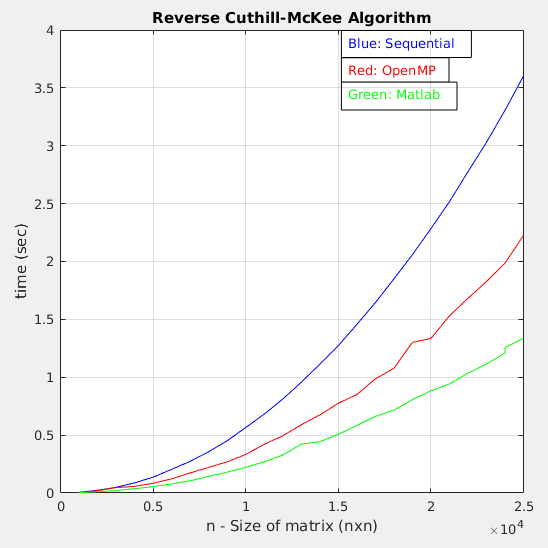
\includegraphics[width=\textwidth]{images/rcm.png}
		\caption{Comparison of different implementations}
		\label{fig:rcm}
	\end{minipage}
	\hfill
	\begin{minipage}[b]{0.45\textwidth}
		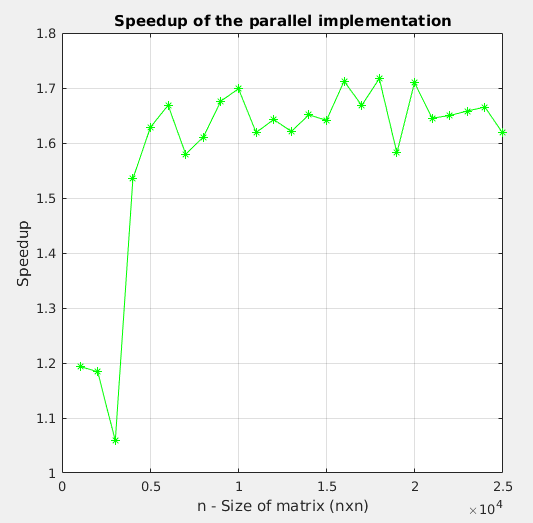
\includegraphics[width=\textwidth]{images/speedup.png}
		\caption{Speedup achieved using OpenMP}
		\label{fig:speedup}
	\end{minipage}
\end{figure}

\section{Observations}
\vspace{2mm} %2mm vertical space

\subsection{Result}
\vspace{2mm} %2mm vertical space

From the images below, one can observe that this RCM implementation is an accurate one, since it's almost the same result as matlab, which for is valid. This specific test was made for n=10000 and density=0.1\%.

\begin{figure}[!htb]

	\begin{minipage}[b]{0.32\textwidth}
		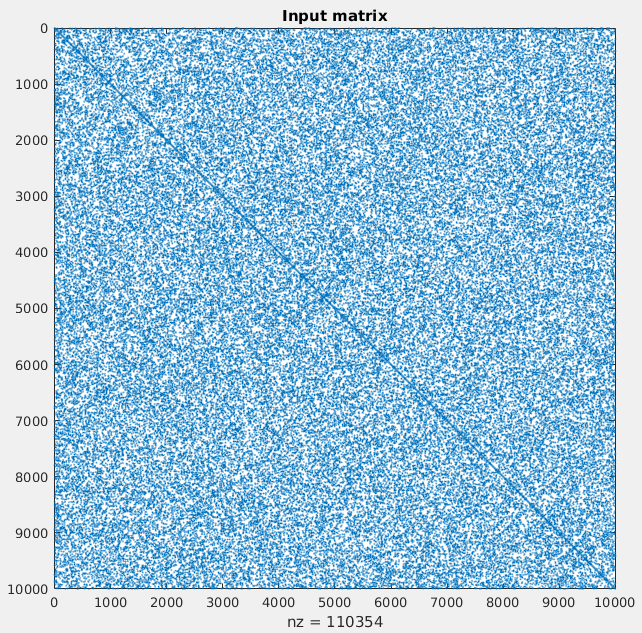
\includegraphics[width=\textwidth]{images/input.png}
		\caption{Input matrix (n=10000 , density = 0.1\%)}
		\label{fig:input}
	\end{minipage}
	\hfill
	\begin{minipage}[b]{0.32\textwidth}
		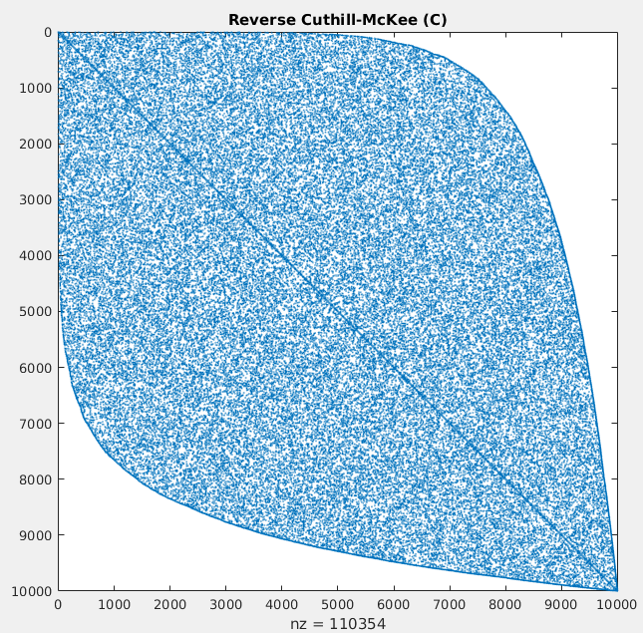
\includegraphics[width=\textwidth]{images/out_c.png}
		\caption{Output achieved with C}
		\label{fig:output_c}
	\end{minipage}
	\hfill
	\begin{minipage}[b]{0.32\textwidth}
		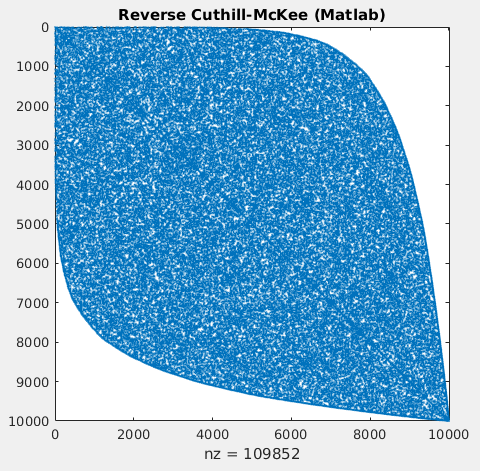
\includegraphics[width=\textwidth]{images/out_matlab.png}
		\caption{Output achieved with Matlab}
		\label{fig:output_matlab}
	\end{minipage}
\end{figure}

\subsection{Comments}
\vspace{2mm} %2mm vertical space

After observations over the speedup for various parallelizations, it was concluded that the only parts worth parallelizing are two, which are actually responsible for almost 70\% of the total execution time. Despite them only being two, one can clearly see that OpenMP gave a great speedup indeed (35-40\% faster). Although, Matlab implementation is even faster than the parallel one. Also parallel computing is used only at \textbf{n} values higher than the thresholds for both cases (1000 and 2000 accordingly), because for small matrices, sequential implementation is faster than the parallel one.

%++++++++++++++++++++++++++++++++++++++++
% References section will be created automatically 
% with inclusion of "thebibliography" environment
% as it shown below. See text starting with line
% \begin{thebibliography}{99}
% Note: with this approach it is YOUR responsibility to put them in order
% of appearance.

\begin{thebibliography}{99}

\bibitem{ciprian} \emph{Tutorial: Bandwidth reduction - The CutHill-McKee Algorithm},  available at \\
\url{http://ciprian-zavoianu.blogspot.com/2009/01/project-bandwidth-reduction.html}
	
\bibitem{geeksforgeeks} \emph{Reverse Cuthill Mckee Algorithm},  available at \\
\url{https://www.geeksforgeeks.org/reverse-cuthill-mckee-algorithm}

\bibitem{fsu} \emph{Reverse Cuthill McKee Ordering},  available at \\
\url{https://people.sc.fsu.edu/~jburkardt/cpp_src/rcm/rcm.html}
	
\end{thebibliography}

\end{document}
